\chapter{Elderly Care Assisted Living System} % Main chapter title

\label{chapter6} % Change X to a consecutive number; for referencing this chapter elsewhere, use \ref{ChapterX}

%----------------------------------------------------------------------------------------
%	SECTION 1
%----------------------------------------------------------------------------------------

\section{Introduction}


Elderly care has been addressed by many EU-funded research projects since the aging population is one of the main issues the EU is facing. 
There are many solutions to this problem.
One approach is invasive such as wearables, sound sensors, IR occupancy detectors, etc. 
This approach has been addressed by thousands of publications, such as reviews \cite{elderReview1}, \cite{elderReview2} and \cite{elderReview3} show and present.

Authors \cite{elderNILM} and \cite{elderNILMDementia} tried to solve this issue using a non-invasive approach with NILM algorithms. 
In the case of a non-invasive approach, no additional meters need to be installed, since per-appliance usage can be disaggregated.
While this is practical from the "no additional equipment needed" side, it is a bit less practical from the efficiency and accuracy side, especially for larger buildings. 

There is a middle way between invasive and non-invasive approaches, such as the authors explored in paper \cite{elder1} and \cite{elder2}. 
It is possible to use sub-meters for each appliance and indirectly observe the usage pattern. 
The advantage of this approach is that the elder does not need to wear the device.
The disadvantage is, that new meters need to be installed for the most commonly used appliances.
Our approach will use the latter.

\section{Goal}

The chapter will focus on building an elderly care system that will use users' periodic usage patterns to detect an anomaly.
The anomaly could be anything from a fall, stroke or altered usage pattern due to dementia. 
The algorithm will be designed based on the LP \ref{fig:PHPA}, which we discussed in Chapter \ref{chapter4}.
Figure shows, that the first thing in the morning used are a kettle and toaster, and with a delay of one hour, microwave and TV. 
If none of these appliances are used within that hour, then that hour is considered anomalous.
This means that the algorithm will be able to detect the anomaly within 1 hour of the accident.

\section{Methodology}

\subsection{Defining an Anomaly}

Since the elderly care system is based on anomaly detection, we have to define it first.
In our case, the anomaly occurs when something that should operate, does not. 
Based on this definition we will develop an anomaly detection algorithm. 

\subsection{Building Anomaly Detection Algorithm}

The next section will present the steps taken while designing this algorithm.

\subsubsection{Step One}
To detect the anomalies one first needs to build a daily activation profile for each appliance, such as the one previously shown in Figure \ref{fig:PHPA}.
In this specific case, we will be using 2h buckets, yielding a total of 12 buckets. 

\subsubsection{Step Two}
The second step is to ignore appliances that are always on by calculating the standard deviation of activations for each bucket. 
The activations are normalized between 0 and 1. 
This step is important so that appliances that are always on, such as fridges or freezers get ignored. 
These appliances are detected based on the width of their activation normal distribution. 
Periodic (on an hourly basis) appliances should have narrow distributions and the more dynamic should have wider distributions.
This can be seen in examples from building 2.
\begin{figure}[H]
    \centering
    \begin{tikzpicture}
        \coordinate (s) at (0,0);
        \foreach \num in {866, 842, 810, 772, 868, 854, 859, 854, 864, 887, 889, 883}{
        \node[minimum size=6mm, draw, rectangle] at (s) {\num};
        \coordinate (s) at ($(s) + (1,0)$);
        }
    \end{tikzpicture}
    \caption{Daily activations for fridge $\sigma$ = 0.036}
    \label{arr:fridge_acts}
\end{figure}

\begin{figure}[H]
    \centering
    \begin{tikzpicture}
        \coordinate (s) at (0,0);
        \foreach \num in {86, 77, 75, 74, 100, 118, 113, 127, 168, 202, 171, 121}{
        \node[minimum size=6mm, draw, rectangle] at (s) {\num};
        \coordinate (s) at ($(s) + (1,0)$);
        }
    \end{tikzpicture}
    \caption{Daily activations for audio system $\sigma$ = 0.2}
    \label{arr:as_acts}
\end{figure}

\begin{figure}[H]
    \centering
    \begin{tikzpicture}
        \coordinate (s) at (0,0);
        \foreach \num in {9, 4, 4, 3, 212, 122, 85, 80, 102, 260, 134, 48}{
        \node[minimum size=6mm, draw, rectangle] at (s) {\num};
        \coordinate (s) at ($(s) + (1,0)$);
        }
    \end{tikzpicture}
    \caption{Daily activations for microwave $\sigma$ = 0.3}
    \label{arr:microwave_acts}
\end{figure}

Based on results from all appliances a threshold of $\sigma$ = 0.1 was set.
This method will also get rid of appliances that are always on due to their specific nature such as server computers 
or fridges. 

\subsubsection{Step Three}

Next, appliances that trigger together must be grouped. 
This means we must find part of the day that they are operating together.
Due to the filter in the previous step, we are left with appliances whose usage variate throughout the day. 
Some appliances are on even when the user is not necessarily using them, this can be seen in figure \ref{arr:as_acts}.
One of many ways to do this is to normalize the activations, this yields a metric that tells us the probability of that appliance being turned on compared to the rest of the day. 
If we do this for the same appliances as above the result is the following: 

\begin{figure}[H]
    \centering
    \begin{tikzpicture}
        \coordinate (s) at (0,0);
        \foreach \num in {0.43, 0.38, 0.37, 0.37, 0.5 , 0.58, 0.56, 0.63, 0.83, 1. , 0.85,
        0.6}{
        \node[minimum size=6mm, draw, rectangle] at (s) {\num};
        \coordinate (s) at ($(s) + (1,0)$);
        }
    \end{tikzpicture}
    \caption{Daily activations for audio system $\sigma$ = 0.2}
    \label{arr:as_acts_norm}
\end{figure}

\begin{figure}[H]
    \centering
    \begin{tikzpicture}
        \coordinate (s) at (0,0);
        \foreach \num in {0.03, 0.02, 0.02, 0.01, 0.82, 0.47, 0.33, 0.31, 0.39, 1.  , 0.52,
        0.18}{
        \node[minimum size=6mm, draw, rectangle] at (s) {\num};
        \coordinate (s) at ($(s) + (1,0)$);
        }
    \end{tikzpicture}
    \caption{Daily activations for microwave $\sigma$ = 0.3}
    \label{arr:microwave_acts_norm}
\end{figure}

Finally, a suitable threshold must be selected.
The threshold of 0.5 was selected, which yields the following vectors:

\begin{figure}[H]
    \centering
    \begin{tikzpicture}
        \coordinate (s) at (0,0);
        \foreach \num in {0, 0, 0, 0, 0, 1, 1, 1, 1, 1, 1, 1}{
        \node[minimum size=6mm, draw, rectangle] at (s) {\num};
        \coordinate (s) at ($(s) + (1,0)$);
        }
    \end{tikzpicture}
    \caption{Daily activations for audio system}
    \label{arr:as_acts_vec}
\end{figure}

\begin{figure}[H]
    \centering
    \begin{tikzpicture}
        \coordinate (s) at (0,0);
        \foreach \num in {0, 0, 0, 0, 1, 0, 0, 0, 0, 1, 1, 0}{
        \node[minimum size=6mm, draw, rectangle] at (s) {\num};
        \coordinate (s) at ($(s) + (1,0)$);
        }
    \end{tikzpicture}
    \caption{Daily activations for microwave with one usage peak in the morning and the other in the evening}
    \label{arr:microwave_acts_vec}
\end{figure}

The vectors show us that the microwave has two usage peaks, where the audio system can be used anytime throughout the day.
It is possible to do this for all appliances, which results in a 2D matrix. 
Using this matrix we can build rules for which appliances are being used together.
Figure \ref{arr:act_mat} uses rows for appliances and columns for buckets.  
If we use terminology from image processing the matrix \ref{arr:act_mat} is essentially a highly saturated LP \ref{fig:PHPA},
which can be easily processed by computer algorithms due to binary encoding. 

\begin{figure}[H]
    \centering
    \begin{tikzpicture}
        \coordinate (s) at (0,8);
        \foreach \num in {0, 0, 0, 0, 0, 1, 1, 1, 1, 1, 1, 1}{
        \node[minimum size=6mm, draw, rectangle] at (s) {\num};
        \coordinate (s) at ($(s) + (1,0)$);
        }
        \coordinate (s) at (0,7);
        \foreach \num in {0, 0, 0, 0, 0, 0, 0, 0, 0, 1, 1, 1}{
        \node[minimum size=6mm, draw, rectangle] at (s) {\num};
        \coordinate (s) at ($(s) + (1,0)$);
        }
        \coordinate (s) at (0,6);
        \foreach \num in {0, 0, 0, 0, 0, 0, 0, 0, 1, 1, 0, 0}{
        \node[minimum size=6mm, draw, rectangle] at (s) {\num};
        \coordinate (s) at ($(s) + (1,0)$);
        }
        \coordinate (s) at (0,5);
        \foreach \num in {0, 0, 0, 0, 0, 0, 0, 0, 0, 0, 0, 0}{
        \node[minimum size=6mm, draw, rectangle] at (s) {\num};
        \coordinate (s) at ($(s) + (1,0)$);
        }
        \coordinate (s) at (0,4);
        \foreach \num in {0, 0, 0, 0, 1, 0, 0, 1, 1, 1, 1, 0}{
        \node[minimum size=6mm, draw, rectangle] at (s) {\num};
        \coordinate (s) at ($(s) + (1,0)$);
        }
        \coordinate (s) at (0,3);
        \foreach \num in {0, 0, 0, 0, 1, 1, 0, 0, 1, 0, 0, 0}{
        \node[minimum size=6mm, draw, rectangle] at (s) {\num};
        \coordinate (s) at ($(s) + (1,0)$);
        }
        \coordinate (s) at (0,2);
        \foreach \num in {0, 0, 0, 0, 1, 1, 0, 1, 0, 0, 0, 0}{
        \node[minimum size=6mm, draw, rectangle] at (s) {\num};
        \coordinate (s) at ($(s) + (1,0)$);
        }
        \coordinate (s) at (0,1);
        \foreach \num in {0, 0, 0, 0, 1, 0, 1, 0, 0, 0, 1, 0}{
        \node[minimum size=6mm, draw, rectangle] at (s) {\num};
        \coordinate (s) at ($(s) + (1,0)$);
        }
        \coordinate (s) at (0,0);
        \foreach \num in {0, 0, 0, 0, 0, 1, 1, 1, 1, 1, 0, 0}{
        \node[minimum size=6mm, draw, rectangle] at (s) {\num};
        \coordinate (s) at ($(s) + (1,0)$);
        }
    \end{tikzpicture}
    \caption{Activation matrix}
    \label{arr:act_mat}
\end{figure}

It is possible to display the matrix \ref{arr:act_mat} as an image.
The Figure below shows how the LP is transformed.

\begin{figure}[H]
	\begin{subfigure}{.5\textwidth}
		% \centering
		\caption{Input data}
		\includegraphics[width=1\linewidth]{../Figures/LPS/PHPA_profile_for_building.pdf}
		\label{fig:ec_PHPA}
	\end{subfigure}%
	~ 
	\begin{subfigure}{.5\textwidth}
		% \centering
		\caption{Figure \protect\ref{arr:act_mat} as an image}
		\includegraphics[width=1\linewidth]{../Figures/LPS/PHPA_EC.png}
		\label{fig:ec_PHPA_bw}
	\end{subfigure}%

	\caption{Transformation of source LP to black and white}
\end{figure}

\subsubsection{Step Four}

Previously, we have defined that an anomaly occurs when something that should activate does not.
Using the matrix \ref{arr:act_mat} we can compile an algorithm that will detect the anomaly using current activations being tested 
and comparing it to the adjacent column in matrix \ref{arr:act_mat}.
Let us use the fifth bucket as an example. That is data from 8 to 10 o'clock.

The tested sample is considered normal if at least two appliances that are normally being used are activated.
Otherwise, the tested sample is considered anomalous.
Our implementation multiplies the adjacent matrix column to the tested sample.
We sum the elements of the resulting array and check if it is larger or equal to 2.
If cases where this rule is false, samples are considered anomalous.

\begin{figure}[H]
    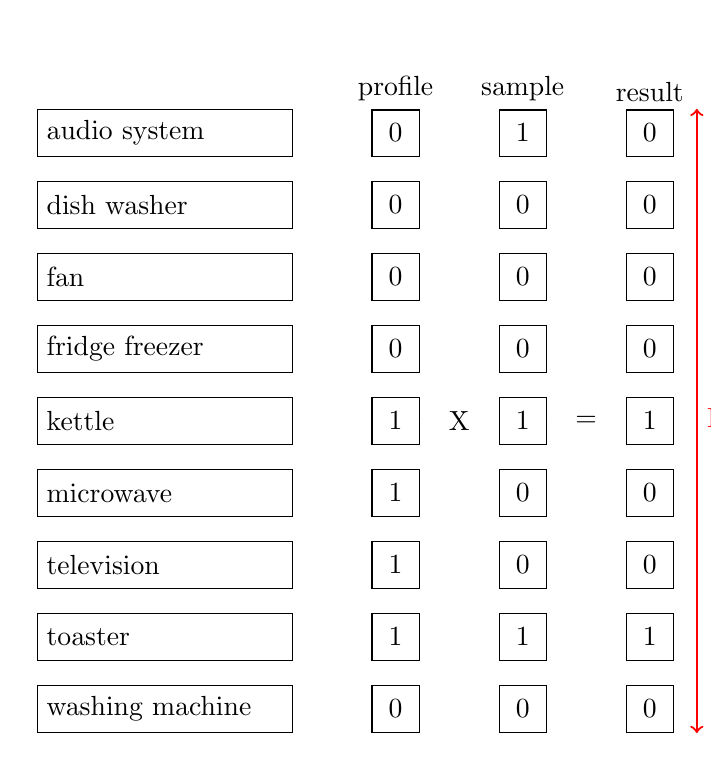
\begin{tikzpicture}
      \matrix [row sep=3mm, column sep=1cm,nodes={minimum size=6mm, draw, rectangle}]
      {
      \node[text width=3cm,white] {margin};\\ 
      \node[text width=3cm] {audio system}; &  \node (t1){0}; & \node  (t2){1}; & \node (s1){0};\\
      \node[text width=3cm] {dish washer}; &   \node     {0}; & \node     {0}; & \node     {0};\\
      \node[text width=3cm] {fan}; &           \node     {0}; & \node     {0}; & \node     {0};\\
      \node[text width=3cm] {fridge freezer}; &\node     {0}; & \node     {0}; & \node     {0};\\
      \node[text width=3cm] {kettle}; &        \node (a) {1}; & \node (b) {1}; & \node (c) {1};\\
      \node[text width=3cm] {microwave}; &     \node     {1}; & \node     {0}; & \node     {0};\\
      \node[text width=3cm] {television}; &    \node     {1}; & \node     {0}; & \node     {0};\\
      \node[text width=3cm] {toaster}; &       \node     {1}; & \node     {1}; & \node     {1};\\
      \node[text width=3cm] {washing machine}; &\node    {0}; & \node     {0}; & \node (s2){0};\\
      };
      \draw [<->,white] (a.east) -- (b.west) node[black] [midway] {X};
      \draw [<->,white] (b.east) -- (c.west) node[black] [midway] {=};
    
      \begin{scope}[transform canvas={yshift=0.8em}]
      \draw [-] (t1.west) -- (t1.east)node[black] [above,midway] {profile};
      \end{scope}  
    
      \begin{scope}[transform canvas={yshift=0.8em}]
      \draw [-] (t2.west) -- (t2.east)node[black] [above,midway] {sample};
      \end{scope}
    
      \begin{scope}[transform canvas={yshift=0.8em}]
      \draw [-] (s1.west) -- (s1.east)node[black] [above,midway] {result};
      \end{scope}
    
      \begin{scope}[transform canvas={xshift=1.7em}]
       \draw [<->,red,thick] (s1.north) -- (s2.south) node [right,midway] {IF SUM >= 2 not an anomaly};
      \end{scope}
    \end{tikzpicture}
    \caption{The evaluation of the test sample compared to the adjacent column from the matrix. An example is for a fifth bucket or fifth row from the matrix.}
    
\end{figure}

% \begin{figure}[H]
%     \centering
%     \caption{Process of evaluating an anomaly}
%     \includegraphics[width=1\linewidth]{../Figures/EC/EC_anom_dect.png}
%     \label{fig:anom_detct}
%     \caption{The evaluation of new bucket compared to matrix. An example is for a fifth bucket or fifth row from the matrix.}
    
% \end{figure}

This process is done for all samples, where we count normal and anomalous samples for each bucket
The important thing to note here is that we are evaluating the samples from train data, from which the profile was built.

\begin{figure}[H]
    \centering
    \begin{tikzpicture}
        \coordinate (s) at (0,0);
        \foreach \num in {472, 469, 468, 466, 57, 153, 288, 187, 123, 84, 75, 281}{
        \node[minimum size=6mm, draw, rectangle] at (s) {\num};
        \coordinate (s) at ($(s) + (1,0)$);
        }
    \end{tikzpicture}
    \caption{Aggregated anomalies for each bucket}
    \label{arr:agg_anom}
\end{figure}

\begin{figure}[H]
    \centering
    \begin{tikzpicture}
        \coordinate (s) at (0,0);
        \foreach \num in {0, 0, 0, 0, 409, 312, 181, 280, 342, 384, 394, 188}{
        \node[minimum size=6mm, draw, rectangle] at (s) {\num};
        \coordinate (s) at ($(s) + (1,0)$);
        }
    \end{tikzpicture}
    \caption{Aggregated normal samples for each bucket}
    \label{arr:agg_norm}
\end{figure}

\subsubsection{Step Five}

The next step is to combine these two arrays so that we calculate the percentage of anomalous samples 
for each bucket with an equation. 

\begin{equation}
    \frac{N_{anom}}{N_{anom}+N_{norm}}
    \label{eq:ratio}
\end{equation}

Where $N_{anom}$ is a number of anomalous samples and $N_{norm}$ is a number of normal samples.


We can alter the Equation \ref{eq:ratio} so that it will measure
a number of normal samples out of all. 
The result is the Equation \ref{eq:routine}
In other words, we are measuring the strength of a routine that 
user has in each bucket.

\begin{equation}
    R_{outine}= \frac{N_{norm}}{N_{anom}+N_{norm}}
    \label{eq:routine}
\end{equation}

Using the Equation \ref{eq:routine} we can populate the array in Figure \ref{arr:anom_ratio}.

\begin{figure}[H]
    \centering
    \begin{tikzpicture}
        \coordinate (s) at (0,0);
        \foreach \num in {0.0, 0.0, 0.0, 0.0, 0.88, 0.7, 0.39, 0.6, 0.74, 0.82, 0.84, 0.4}{
        \node[minimum size=6mm, draw, rectangle] at (s) {\num};
        \coordinate (s) at ($(s) + (1,0)$);
        }
    \end{tikzpicture}
    \caption{Aggregated anomalies for each bucket}
    \label{arr:anom_ratio}
\end{figure}

In other words, the array in Figure \ref{arr:anom_ratio} tells us how persistent is the user's routine in each bucket or part of the day. 
The higher the metric the higher the routine. 
Since routine is detected based on the usage of appliances it cannot be picked up during the night.

It is possible to see that the routine is quite high during the morning and evening hours.
The anomaly detection algorithm will work best when the metric above is high.
A good trait of the elderly is that their routine is quite high even during the day.

One more thing to do is to ignore the parts of the day when the user has no routine.
This is done by using the array in Figure \ref{arr:anom_ratio} and setting a threshold of 0.7. 

A threshold of 0.5 would mean that we could detect false positive anomalies every other day.
Setting the rate to 0.7 reduces this to every third day.
Here, compromises must be made, the lower the threshold the more accurate the algorithm will be. 
This also means that it will be less sensitive. 
In our case, there is not much harm in false positive detections, since the caregiver can call the elder to check if it is okay.  

\begin{figure}[H]
    \centering
    \begin{tikzpicture}
        \coordinate (s) at (0,0);
        \foreach \num in {0, 0, 0, 0, 1, 1, 0, 0, 1, 1, 1, 0}{
        %\foreach \num in {1.0, 1.0, 1.0, 1.0, 0.12, 0.3, 0.61, 0.4, 0.26, 0.18, 0.16, 0.6}{
        \node[minimum size=6mm, draw, rectangle] at (s) {\num};
        \coordinate (s) at ($(s) + (1,0)$);
        }
    \end{tikzpicture}
    \caption{Using the above-mentioned threshold a new mask is made, to check only buckets with high routine.}
    \label{arr:anom_ratio_mask}
\end{figure}

\subsubsection{Step Six}

The last step is to repeat steps 4 and 5 with test data.
When using test data, we skip the buckets with low routine rates by using the mask on Figure \ref{arr:anom_ratio_mask}.
Since the profile has never seen the data being used, this should give us a good presentation of actual performance in a real-world scenario.

\subsection{The metric - routine rate}

Due to the lack of ground truth data of actual accidents, it is hard to determine the 
exact accuracy of this algorithm. Every anomaly detected is not necessarily an 
actual accident, it could be that the user decided to lie in bed a bit longer, or decided to go to bed early in the evening.
One metric that we can use to determine how well the algorithm functions is the routine rate metric \ref{arr:anom_ratio}.
The reason behind that is, that if the routine rate is high it means that it will be easier to detect the actual anomaly.

\begin{itemize}
	\item Routine rate of 0 would mean that for that bucket household has no routine at all.
    \item Routine rate of 0.5 would mean that the routine is broken every second day.
    \item Routine rate of 0.8 would mean that routine is broken on average every fifth day.
    \item Routine rate of 1 would mean that this household has a routine that is never broken. 
\end{itemize}

An example of when a user routine rate is close to 1. When a true anomaly occurs such as a fall, the dweller, though he had the same strong routine for the past year, would not be able to practice it, and the algorithm will be quite sure that this is an actual anomaly.
Therefore, the lower the routine rate the less sure we are that an actual anomaly such as a fall occurred.
This is a good alternative measurement, that tells us how well this algorithm will perform. 
Since sometimes it is easier to read when results are presented with percentages, we will sometimes use this way of presenting it.
 
\section{Results} 

Results were obtained for 3 datasets. 
REDD and iAWE datasets were not used, since they were too small. 
They contained less than a month of data. 

\subsection{The Routine Rate Over a Period of Time}

In the following sections, we will present how the metric changes over given periods of time.
This will enable us to see that there are patterns that this metric helps reveal. 
Since we have more than a year of training data, this will enable us to see how the metric changes over years.
This enables us to see how routine changes over the year. 
We cannot use testing data in this case, since there is not enough of it.

\subsubsection{The Routine Rate Through the Week} \label{sssec:ratio_week}

As the behavior of the dweller changes, so does the accuracy of the algorithm. 
One observation that was made, was that the routine was higher during the week than during the weekends,
as can be seen in the Figure \ref{fig:ec_week} below. 
The only exception is Figure \ref{fig:ec_b5week}, which shows that the observation does not hold for all houses. 

\begin{figure}[H]
	\begin{subfigure}{.5\textwidth}
		% \centering
		\caption{Building 2}
		\includegraphics[width=1\linewidth]{../Figures/EC/b2week.pdf}
		\label{fig:ec_b2week}
	\end{subfigure}%
	~ 
	\begin{subfigure}{.5\textwidth}
		% \centering
		\caption{Building 19}
		\includegraphics[width=1\linewidth]{../Figures/EC/b19week.pdf}
		\label{fig:ec_b19week}
	\end{subfigure}%
    \bigskip

    \begin{subfigure}{.5\textwidth}
		% \centering
		\caption{Building 18}
		\includegraphics[width=1\linewidth]{../Figures/EC/b18week.pdf}
		\label{fig:ec_b18week}
	\end{subfigure}%
    ~ 
    \begin{subfigure}{.5\textwidth}
		% \centering
		\caption{Building 5}
		\includegraphics[width=1\linewidth]{../Figures/EC/b5week.pdf}
		\label{fig:ec_b5week}
	\end{subfigure}%
	\caption{Routine rate through the week (train data)}
    \label{fig:ec_week}
\end{figure}


Since we are dealing with the elderly, they have a higher routine, and it does not change that much during the weekends. 
Usually, assisted living systems are put in place since elders are alone in the dwelling.
Taking all of this into account, we could assume that the routine of the elderly is the same trough the week and simply ignore the weekends. 
This should yield more relevant results. 

\subsubsection{Routine Rate Through a Year}

The rate at which the routine is being practiced also changes over a year. 
While on average the routine rate is higher during the winter, spring and fall, it is lower during the summer, due to vacation. 
This can be seen in Figure \ref{fig:ec_year} below. 
It is possible to observe dips in routine. 
In some cases, these dips occur in summer and others in springtime. 
Without metadata, we cannot know for sure, what was the event behind these dips. 
There is a high chance most of them are vacations or other events where one or more dwellers are away from home for extended periods of time. 

\begin{figure}[H]
	\begin{subfigure}{.5\textwidth}
		% \centering
		\caption{Building 2}
		\includegraphics[width=1\linewidth]{../Figures/EC/b2year.pdf}
		\label{fig:ec_b2year}
	\end{subfigure}%
	~ 
	\begin{subfigure}{.5\textwidth}
		% \centering
		\caption{Building 19}
		\includegraphics[width=1\linewidth]{../Figures/EC/b19year.pdf}
		\label{fig:ec_b19year}
	\end{subfigure}%
    \bigskip

    \begin{subfigure}{.5\textwidth}
		% \centering
		\caption{Building 18}
		\includegraphics[width=1\linewidth]{../Figures/EC/b18year.pdf}
		\label{fig:ec_b18year}
	\end{subfigure}%
    ~ 
    \begin{subfigure}{.5\textwidth}
		% \centering
		\caption{Building 5}
		\includegraphics[width=1\linewidth]{../Figures/EC/b5year.pdf}
		\label{fig:ec_b5year}
	\end{subfigure}%
	
	\caption{Routine through the year (train data)}
    \label{fig:ec_year}
\end{figure}

\subsubsection{Effectiveness of Anomaly Detection Through the Day}

The following subsection will show how the effectiveness of anomaly detection changes throughout the day.

One thing to keep in mind is that this algorithm can detect anomalies only when
the routine is high, and when more than two appliances are used in given buckets.

Figure \ref{fig:ignored_buckets_22} shows which buckets are most commonly used for the detection of an anomaly.
The Figure includes averaged values from all buildings and datasets. 
In other words, the Figure presents how strong is average routine throughout the day.

This means that the higher the routine, the higher the chance that this bucket will be used for anomaly detection.
During the night, it is possible to see that the average routine rate is quite high.
This can be seen in Figure \ref{fig:ignored_buckets_22}
this is because most users are routinely sleeping during that period.
As we can see in Figure \ref{fig:ignored_buckets_22},
the high routine rate does not necessarily mean the buckets are useful.


\begin{figure}[H]
	\begin{subfigure}{.5\textwidth}
        \caption{Effectivity of anomaly detection through the day}
        \includegraphics[width=1\textwidth]{Figures/EC/ignored_buckets_dist.pdf}
        \label{fig:ignored_buckets_22}
    \end{subfigure}
    ~
    \begin{subfigure}{.5\textwidth}
        \caption{Actual effectiveness of anomaly detection through the day}
        \includegraphics[width=1\textwidth]{Figures/EC/all_ignored_buckets_dist_incl_act.pdf}
        \label{fig:ignored_buckets_act}
    \end{subfigure}
\end{figure}

To find the usable buckets, an additional filter must be applied.
The rule is that at least two appliances must be commonly used in that bucket. 
After applying this rule the following Figure emerges \ref{fig:ignored_buckets_act}

Figure \ref{fig:ignored_buckets_act} shows that there are two peaks.
One in the morning and the other, a wider one, in the evening.

This means that on an average home the algorithm would perform best in the morning and evening because the average person is at school or work during noon. 
The elderly, are usually at home at noon, which could extend the effective detection window.


\subsubsection{The Anomaly Detection During the Night}

We have seen that anomalies can be detected throughout the day,
but are hard to detect through the night, since appliances are off.

This is because, in our current state, an anomaly occurs when something that should operate, does not.
When the user is sleeping, an anomaly occurs when something that shouldn't operate, does. 
To implement this additional rule, we would have to build two models.
One would be online during the day, and the other when the user is sleeping.

To obtain information about the user's sleep schedule, we could either have a schedule obtained from the user or we could extract it based on the usage pattern of appliances.
It is possible to detect when most of the appliances are inactive and build a sleep profile based on this information.

Using the sleep schedule, it is possible to switch between the two operating modes. 
This new implementation would further extend the time windows within which we can detect the anomalies and thus further improve users' safety.

The main issue is not the detection itself but efficiently detecting
when the user is sleeping. 

The examples above were a demonstration and a look into data and metrics. 
The examples shown were trained and evaluated on the same data. 
To show true performance, we will use test data to determine the actual performance. 


\subsection{Per-Building Results}
\subsubsection{REFIT}

Results show, that the method is on average \textbf{79.3} \% efficient for REFIT.  
In Figure \ref{fig:refit_res} it is possible to see that building 10 and 20 yields much worse results than the rest.
The whole routine pattern is very similar to the Figure \ref{fig:tsne_euclidian} from t-SNE chapter where we calulcated the final euclidian distance between samples of the t-SNE plot.
We will make a deeper analysis of this connection in the last Section \ref{sec:tsne_ec_corr} of this Chapter.


\begin{figure}[H]
	\begin{subfigure}{.5\textwidth}
        \caption{All buildings}
        \includegraphics[width=1\textwidth]{Figures/EC/refit_res.pdf}
        \label{fig:refit_res}
    \end{subfigure}
    ~
    \begin{subfigure}{.5\textwidth}
        \caption{Results for REFIT weekday only}
        \includegraphics[width=1\textwidth]{Figures/EC/refit_res_nw_1.pdf}
        \label{fig:refit_res_nw_1}
    \end{subfigure}
\end{figure}

As mentioned in the sub-sub Section \ref{sssec:ratio_week}, the average routine is different during the week and on weekends.
The assumption was that the routine of elderly people does not change significantly over the week, therefore results should be more relevant if we ignore the weekends.
The results in Figure \ref{fig:refit_res_nw_1} show that the result improved to \textbf{77.08} \%.
If we remove the weekend data, the results improved by \textbf{1} \%. 

\subsubsection{UK-DALE}

As mentioned in Section \ref{ssec:ds_eval}, the UK-DALE is not as big and clean of errors as the previous dataset, so the results could be less relevant.
The results in Figure \ref{fig:ukdale_res}, show that the average result is 74.48 \%. 

\begin{figure}[H]
	\begin{subfigure}{.5\textwidth}
        \caption{Results for UK-DALE}
        \includegraphics[width=1\textwidth]{Figures/EC/ukdale_res.pdf}
        \label{fig:ukdale_res}
    \end{subfigure}
    ~
    \begin{subfigure}{.5\textwidth}
        \centering
        \caption{Results for UK-DALE omitting weekends}
        \includegraphics[width=1\textwidth]{Figures/EC/ukdale_nw_res.pdf}
        \label{fig:ukdale_res_nw}
    \end{subfigure}
\end{figure}


In this case, when we omit the weekend data, we improve the routine just slightly to \textbf{74.51} \%.
There are many reasons behind such small improvement, one of them being that the existing routine of these buildings does not change throughout the weekend. 

\subsubsection{ECO}

ECO is of a similar quality as UK-DALE when taking into account the number of buildings and the length of data, as can be seen in Section \ref{ssec:ds_eval}.
The results in Figure \ref{fig:eco_res}, show that this dataset performed the best, with results of 83.80 \%.
The same as before we can omit weekend data, which can be seen in Figure \ref{fig:eco_res_nw}. This brings the result up to 84.09 \%. 

\begin{figure}[H]
	\begin{subfigure}{.5\textwidth}
        \caption{Results for ECO}
        \includegraphics[width=1\textwidth]{Figures/EC/eco_res.pdf}
        \label{fig:eco_res}
    \end{subfigure}
    ~ 
    \begin{subfigure}{.5\textwidth}
        \caption{Results for ECO omitting weekends}
        \includegraphics[width=1\textwidth]{Figures/EC/eco_res_nw_1.pdf}
        \label{fig:eco_res_nw}
    \end{subfigure}
\end{figure}


\subsection{Combined Results}

After combining results from all 26 buildings, Table \ref{tab:ec_res_weekend} can be populated.
It shows that the algorithm is 79.43 \% efficient at detecting true anomalies. 
On average, the algorithm would label 20.5 \% of samples as false positives, 
in other words, every fifth sample could be a false positive. 

\begin{table}[htbp]
    \centering
    \caption{Combined percentage [\%] of routine rate for 26 buildings}
    \label{tab:ec_res_weekend}
    \begin{tabular}{lcc}
        \hline
        \textbf{including weekend data} & \textbf{test} & \textbf{train} \\
        \hline
        \textbf{mean} & 79.43 & 84.55 \\
        \textbf{std} & 14.62 & 9.05 \\
        \textbf{uncertainty} & 2.81 & 1.74 \\
        \hline
        \end{tabular}
\end{table}

If we assume that average building in our dataset has altered routine trough weekend as can be seen in \ref{fig:ec_week},
and assume that average elder has roughly the same routine throughout the week we can remove the weekend data 
to obtain more relevant results.
Table \ref{tab:ec_res_no_weekend}, shows results after removing weekend data.
We can observe that the mean test routine is 80.42 \%, which is slightly higher compared to results from previous Table \ref{tab:ec_res_weekend}.

\begin{table}[htbp]
    \centering
    \caption{Combined percentage [\%] of routine rate for 26 buildings not including weekend data}
    \label{tab:ec_res_no_weekend}
    \begin{tabular}{lcc}
        \hline
        \textbf{not-including weekend data} & \textbf{test} & \textbf{train} \\
        \hline
        \textbf{mean} & 80.42 & 85.88 \\
        \textbf{std} & 15.58 & 8.25 \\
        \textbf{uncertainty} & 2.99 & 1.58 \\
        \hline
        \end{tabular}
\end{table}

The last rows in Tables \ref{tab:ec_res_no_weekend} and \ref{tab:ec_res_weekend} show uncertainty of our measurements,
which is 2.81 \% for weekend data and 2.99 \% for not including weekend data.

When comparing differences between train and test data it can be clearly observed that train data performed better.
The difference in performance can be attributed to changed user behavior after model was trained.
It would be beneficial if we managed to update the model over time, to include the small changes in users routine.
This will be addressed in the next Section \ref{sec:iter_learning_system}.

\section{Discussion}

The main goal of our system is to detect anomalies when they occur. 
The nature of this system is that there is more harm done if we do not detect an anomaly than if we detect a few false positives. 
On the other hand, too many false positives could lead to caregivers ignoring detections altogether.
In this regard, we must find a balance between the two.
A false positive once a week is a good balance, especially since the care-giver is only a phone call away from checking the status of the patient.
Since the validation is so simple, we can claim that the performance of the system is adequate enough to be used in a real world setting.

When analyzing these results one important to keep in mind is,
that we do not have metadata available to know what kind of socio-economic status dwellers have.
Socio-economic status encompasses attributes such as age, income, number of children, geolocation, etc.
They may also encompass the age of the building, type of insulation, number of dwellers in the buildings, etc.
Since datasets do not provide them, it is hard to make any other conclusions other than the algorithm works well on an average building.

We know that the reason for installing such a system is that the user is left alone.
We can assume that on average there is more than one dweller living in the buildings we tested on.
Since this system would usually be used by a single dweller,
this would be in favor of our algorithm since it would be 
easier to extract the routine.

One other thing that would be in our favor is that the average person spends less time at home than an elderly person. 
If we take a look at the results, it is possible to see that,
the average home has a low routine during the noon. 
This is because the average person is not at home during noon.
This can be seen in Figure \ref{fig:ignored_buckets_22}.
Since the elderly are usually home at that time, this would 
increase the time windows where we can detect the accident.

We could also assume that the older the dweller, the higher the routine. 
The nature of the elderly is that they are more conservative when it comes to changes, and prefer to stick to their routine.
Since the algorithm works better when usage is periodic, this would also be in our favor. 
Taking all of these assumptions into account, 
there is a possibility that this algorithm would work 
better on the elderly due to their nature.
Since the results on the average building are promising
a test study should be performed. 
This would also prove our assumption that this algorithm works 
better on the elderly.

\section{Iterative Learning System}
\label{sec:iter_learning_system}
In the case of practical use of this algorithm, it is 
important the system is put online as fast as possible and that it improves over time. 
This can be achieved with the implementation of iterative learning.
The algorithm will build an LP based on the first month of data.
Using this LP, the system can be immediately put online.
At the end of the month, it can use this data to improve the model, which can then be repeated indefinitely. 
 
\subsection{Methodology}
The tools, metric and other methodology is the same as in a normal learning system.
The only change was made on the data preparation side.

\subsubsection{Data Preparation}
For this evaluation, only REFIT (\cite{REFIT}) data was used. 
As it can be seen in Figure \ref{fig:refit_timeline},
Refit buildings have long and relatively similar timelines,
compared to other datasets.

On Figure \ref{fig:dyn_data_1} it is possible to see,
how the amount of training and testing data changes over 16 months.

\begin{figure}[H]
	\centering
	\caption{Data for building 1 over 16 months}
	\includegraphics[]{Figures/EC/DYN/tst_tr_b1.pdf}
	\label{fig:dyn_data_1}
\end{figure}

We can also plot how the amount of data changes for all buildings.
This can be seen in Figure \ref{fig:data_used_for_training}.

\begin{figure}[H]
	\begin{subfigure}{.5\textwidth}
        \caption{Data used for training}
        \includegraphics[width=1\textwidth]{Figures/EC/DYN/data_used_for_training_all.pdf}
        \label{fig:data_used_for_training}
    \end{subfigure}
    ~
    \begin{subfigure}{.5\textwidth}
        \caption{Data used for training, with removed buildings}
        \includegraphics[width=1\textwidth]{Figures/EC/DYN/data_used_for_training_removed_short.pdf}
        \label{fig:data_used_for_training_removed}
    \end{subfigure}
\end{figure}

To analyze the results, at least 1 year of usable data should be available. 
Figure \ref{fig:data_used_for_training_removed} shows only buildings containing at least one year of data.
Similarly, we can check how test data changes over the months. 
In this case, data is not being aggregated, but only one month of it is used at a time.
Figure \ref{fig:data_used_for_testing} shows, that after one year
the amount of data used for training starts to decline. 
To get more accurate results we will only observe the performance using one year of data. 

\begin{figure}[H]
	\centering
	\caption{Data used for training, with removed buildings}
	\includegraphics[]{Figures/EC/DYN/data_used_for_testing.pdf}
	\label{fig:data_used_for_testing}
\end{figure}

\subsection{Results}

To show the effect of training data on the metric, Figure \ref{fig:efect_of_data_on_metric} is presented.
Figure \ref{fig:efect_of_data_on_metric} contains 12 months of 
data for each house.

\begin{figure}[H]
	\centering
	\caption{Effect of new data on metric}
	\includegraphics[]{Figures/EC/DYN/efect_of_data_on_metric.pdf}
	\label{fig:efect_of_data_on_metric}
\end{figure}

Figure \ref{fig:efect_of_data_on_metric} shows, that in most cases, results converge towards 80 \%. 
In some cases, the results are good from the beginning, but sooner or later the routine rate will dip. 
With more data, these dips become smaller and less frequent. 
If the behavior in the household radically changes, it can still lead to a dip.

\begin{figure}[H]
	\centering
	\caption{Metric over 12 months}
	\includegraphics[]{Figures/EC/DYN/1_year_of_iterative_learning_avg.pdf}
	\label{fig:1_year_of_iterative_learning_avg}
\end{figure}

Figure \ref{fig:1_year_of_iterative_learning_avg} shows how the same data can also be presented so that it shows how the metric changes over a year.
The same as in the previous Figure \ref{fig:efect_of_data_on_metric} we can observe the dips getting less frequent and smaller. 
Here we can also observe the average line. 
The average value seems to be on average at around 80 - 85 \%,

\subsection{Discussion}

It is hard to compare these results from iterative learning to the ones from non-iterative learning.
Even though the same data was used, different sections of it were used.

Let's take the last point in the Figure where the average is at the 85 \% mark for an example.
Here, the amount of training data is different, since we limited it to one year. 
The train set is also different since only last month was used, and not 20 \%. 
There are many differences between train and test sets, therefore we can not compare them.
The results do prove that the method works and that the true performance is at around the expected 80 \%.

By increasing the amount of data, the algorithm becomes more stable.
In some cases, where users' behavior does not change, the algorithm could work
from the first month forward. In other cases, where behavior is more dynamic, 
the algorithm needs a month or two to stabilize. 

It is important to note that the longer the observation, the higher chance there is
that the routine of the user will change.
When such changes do occur, the algorithms must have methods in place, that enable them to adjust to the new routine.
The simplest approach would be to use weights, which put more attention on more recent data and less attention on older data.

Future research could explore these limitations and expand on the findings of the current study.
For example, additional studies could investigate the performance of the algorithm under different conditions or compare it to other methods of anomaly detection. 
Additionally, further research could examine the potential applications and implications of the method, such as how it could be used to improve the safety or efficiency of dwelling systems.

\section{Correlation Between t-SNE Plot Euclidean Distance and Routine Rate}
\label{sec:tsne_ec_corr}
In Section \ref{ssec:tsne_euclidian_distance}, we first observed the presence of periodic behavior in formed t-SNE clusters.
We speculated, that the scattering of LP clusters could be correlated to a routine so that the smaller the scattering the better the routine.
We calculated the scattering using Euclidean distance, the same metric used as a cost function in t-SNE

Figure \ref{fig:tsne_euclidian2} was already presented in Section \ref{ssec:tsne_euclidian_distance},
but it makes sense to reuse it here in this context. 
As mentioned this Figure shows the Euclidean distance between samples for per-building LPs for every building.

\begin{figure}[H]
	\centering
	\caption{Euclidean distance of samples for every building using normalized LPs}
	\includegraphics[]{Figures/EC/CORR_TSNE/tnse_euclidian.pdf}
	\label{fig:tsne_euclidian2}
\end{figure}

To reveal the connection between the two, we plotted both on the same Figure \ref{fig:tsne_comparison}.
The routine rate in this Figure is reused from Figure \ref{fig:refit_res}.

\begin{figure}[H]
	\centering
	\caption{Plot of results from REFIT and t-SNE Euclidean distance }
	\includegraphics[]{Figures/EC/CORR_TSNE/TSNE_EC_comparison.pdf}
	\label{fig:tsne_comparison}
\end{figure}

Figure \ref{fig:tsne_norm} shows the same data as the Figure above, but it's normalized using a min-max scaler.
Additionally, we have inverted the values of Euclidean distance, since values seem to be inversely correlated.
Looking at the Figure it is clear that there is some similarity between the two columns,
especially for the best and worst-performing buildings.

\begin{figure}[H]
	\centering
	\caption{Normalized values}
	\includegraphics[]{Figures/EC/CORR_TSNE/TSNE_EC_norm.pdf}
	\label{fig:tsne_norm}
\end{figure}

To furthermore prove the similarity, we have used the methodological approaches for calculating similarity that we explained in Section \ref{ssec:lp_similarity}.
The results can be observed in Table \ref{tab:similarity_results}.
First, we calculated cosine similarity using Equation \ref{eq:cosine_similarity}, which yielded a cosine similarity of \textbf{0.94}  for the data seen in the second Figure \ref{fig:tsne_comparison} and \textbf{0.86} for data seen in the third Figure \ref{fig:tsne_norm}.
Second, we calculated Pearson's correlation coefficient using Equation \ref{eq:pearson_correlation}, which yielded a result of \textbf{-0.76} for the data seen in the second Figure \ref{fig:tsne_comparison} and \textbf{0.76} for data seen in the third Figure \ref{fig:tsne_norm}.
These values present that there is a connection between the t-SNE plot and the routine of the households.

\begin{table}[ht]
    \centering
    \caption{Similarity and correlation results}
    \label{tab:similarity_results}
    \begin{tabular}{@{}lcc@{}}
    \toprule
    \textbf{Method} & \textbf{Figure \ref{fig:tsne_comparison}} & \textbf{Figure \ref{fig:tsne_norm}} \\ \midrule
    Cosine similarity & 0.94 & 0.86 \\
    Pearson's correlation coefficient & -0.76 & 0.76 \\ \bottomrule
    \end{tabular}
\end{table}

When analyzing these results we must keep in mind that the methodological approaches were very different for the two experiments.
In the case of t-SNE, we have used normalized per-building LPs with very little preprocessing, whereas in the elderly care algorithm, we have used per-building per-appliance LPs with extensive pre-processing to extract appliances that could help us detect the routine.
Another thing we must keep in mind is that elderly care enables us to detect anomalies on hourly intervals, whereas our t-SNE approach needs a minimum of a week of data to construct the LPs.
In this regard, t-SNE could be used to evaluate the routine rate of a household.

\subsection{Discussion}
This connection is an important demonstration that confirms our statements from Chapter \ref{chapter5} that the dispersion of samples in the t-SNE plot is related to routine.
This also means that we can rely on t-SNE to evaluate the routine of a household.
While it may not be as precise and fast as an elderly care algorithm, it is simple to use. 
Apart from implementation being easily available, it uses per-building LPs which can be built off most existing residential power meters.

This leads us to privacy issues, as almost all households use power meters for utility billing tracking. Before processing this data to build per-building LPs, the user should be informed and agree to the use of their data.
It should also be made clear that their data will be handled according to GDPR.

\section{Summary}

The results show that our approach can detect changes in routine and can improve over time.
Due to a lack of gourd truth data, we were not able to measure the exact accuracy of the system,
but rather evaluate if the behavior of residents is sufficiently periodic.
Even the best algorithm would not be able to detect anomalies in a stochastic system.
With that, we also proved that such a system is sufficiently deterministic for such applications.

Furthermore, we have demonstrated the existence of a connection between the t-SNE plot and the routine obtained from the elderly care anomaly detection algorithm.
While t-SNE cannot be directly used in the setting of elderly care, as it's too slow, it could be used to determine if the routine of the household is strong enough before a more complex system is put in place.

